\documentclass{article} % Especially this!

\usepackage[english]{babel}
\usepackage[utf8]{inputenc}
\usepackage[margin=1in]{geometry}
\usepackage{amsmath}
\usepackage{amsthm}
\usepackage{amsfonts}
\usepackage{amssymb}
\usepackage{graphicx}
\usepackage{hyperref}
\usepackage[numbers, square]{natbib}
\usepackage{fancybox}
\usepackage{epsfig}
\usepackage{soul}
\usepackage[framemethod=tikz]{mdframed}
\usepackage[shortlabels]{enumitem}
\usepackage[version=4]{mhchem}
\usepackage{multicol}
\usepackage{graphicx}
\graphicspath{ {./} }

\newcommand{\blah}{blah blah blah \dots}

\setlength{\marginparwidth}{3.4cm}

\newcommand{\summary}[1]{
\begin{mdframed}[nobreak=true]
\begin{minipage}{\textwidth}
\vspace{0.5cm}
\end{minipage}
\end{mdframed}}

\renewcommand*{\thefootnote}{\fnsymbol{footnote}}

\title{
\normalfont \large
\textsc{ASSIGNMENT-1
\vspace{10pt}
\\COP 290, Spring 2021} \\
[10pt]
\rule{\linewidth}{0.5pt} \\[6pt] 
\Large \textbf{Traffic density estimation using OpenCV functions} \\
\rule{\linewidth}{2pt}  \\[10pt]
}
\author{Jitender Kumar Yadav, 2019CS10361
\\Asha Ram Meena, 2019CS10337}
\date{\normalsize \today}
\begin{document}

\maketitle
\section{Subtasks}
\textbf{
\begin{enumerate}
    \item Camera angle correction and frame cropping
    \item Queue and dynamic density estimation from traffic video
    \item Understanding and analyzing trade-offs in software design
\end{enumerate}
}

\section{Algorithm and Approach}
\begin{itemize}
    \item[$\diamond$] \textbf{Sub-task 1.1}
    \begin{itemize}
        \item[$\square$] Four points were selected using mouse forming a vector containing source points.
        \item[$\square$] Four destination points were manually chosen to map the source points to.
        \item[$\square$] The points were mapped using openCV functions to generate a homography matrix.
        \item[$\square$] The source image was angle-corrected and cropped and stored in accordance to the homography matrix.
    \end{itemize}
    \item[$\diamond$] \textbf{Sub-task 1.2}
    \begin{itemize}
        \item[$\square$] The input video was captured and each frame was caught one by one and corrected and cropped in accordance to first sub-task.
        \item[$\square$] The image of empty road was taken and corrected and cropped.
        \item[$\square$] The difference between two images was taken, gray-scaled and threshold was applied to it.
        \item[$\square$] The number of vehicles was counted by considering each contour in the processed image.
        \item[$\square$] For static density, difference of current frame and empty road was taken, while for dynamic density the difference of adjacent frames was considered.
    \end{itemize}
    \item[$\diamond$] \textbf{Sub-task 1.3}
    \begin{itemize}
        \item[$\square$] \textbf{Method 1}: The function to process frames was modified to accommodate skipping some frames while processing. The parameter was modified and utility calculated.
        \item[$\square$] \textbf{Method 2}: The cropped frame was re-scaled to different resolutions and the impact on utility and processing time was measured.
        \item[$\square$] \textbf{Method 3}: The frame was split into some vertical strips and each strip was given to a different thread to process to save time.
        \item[$\square$] \textbf{Method 4}: Frames were grouped and each group was given to a different thread to process.
        \item[$\square$] \textbf{Utility-Trade-off}: The utility function was calculated by taking root mean square of the relative deviations from the queue density measured in the second sub-task. Utility was plotted against time to measure the impact.
    \end{itemize}
\end{itemize}

\section{Input and Output}
The input and output were through console and locally stored text, image and video files. Suitable makefile and readme were provided to facilitate smooth input and output. The output images and the user interfaces are shown as below.

\subsection{Output}
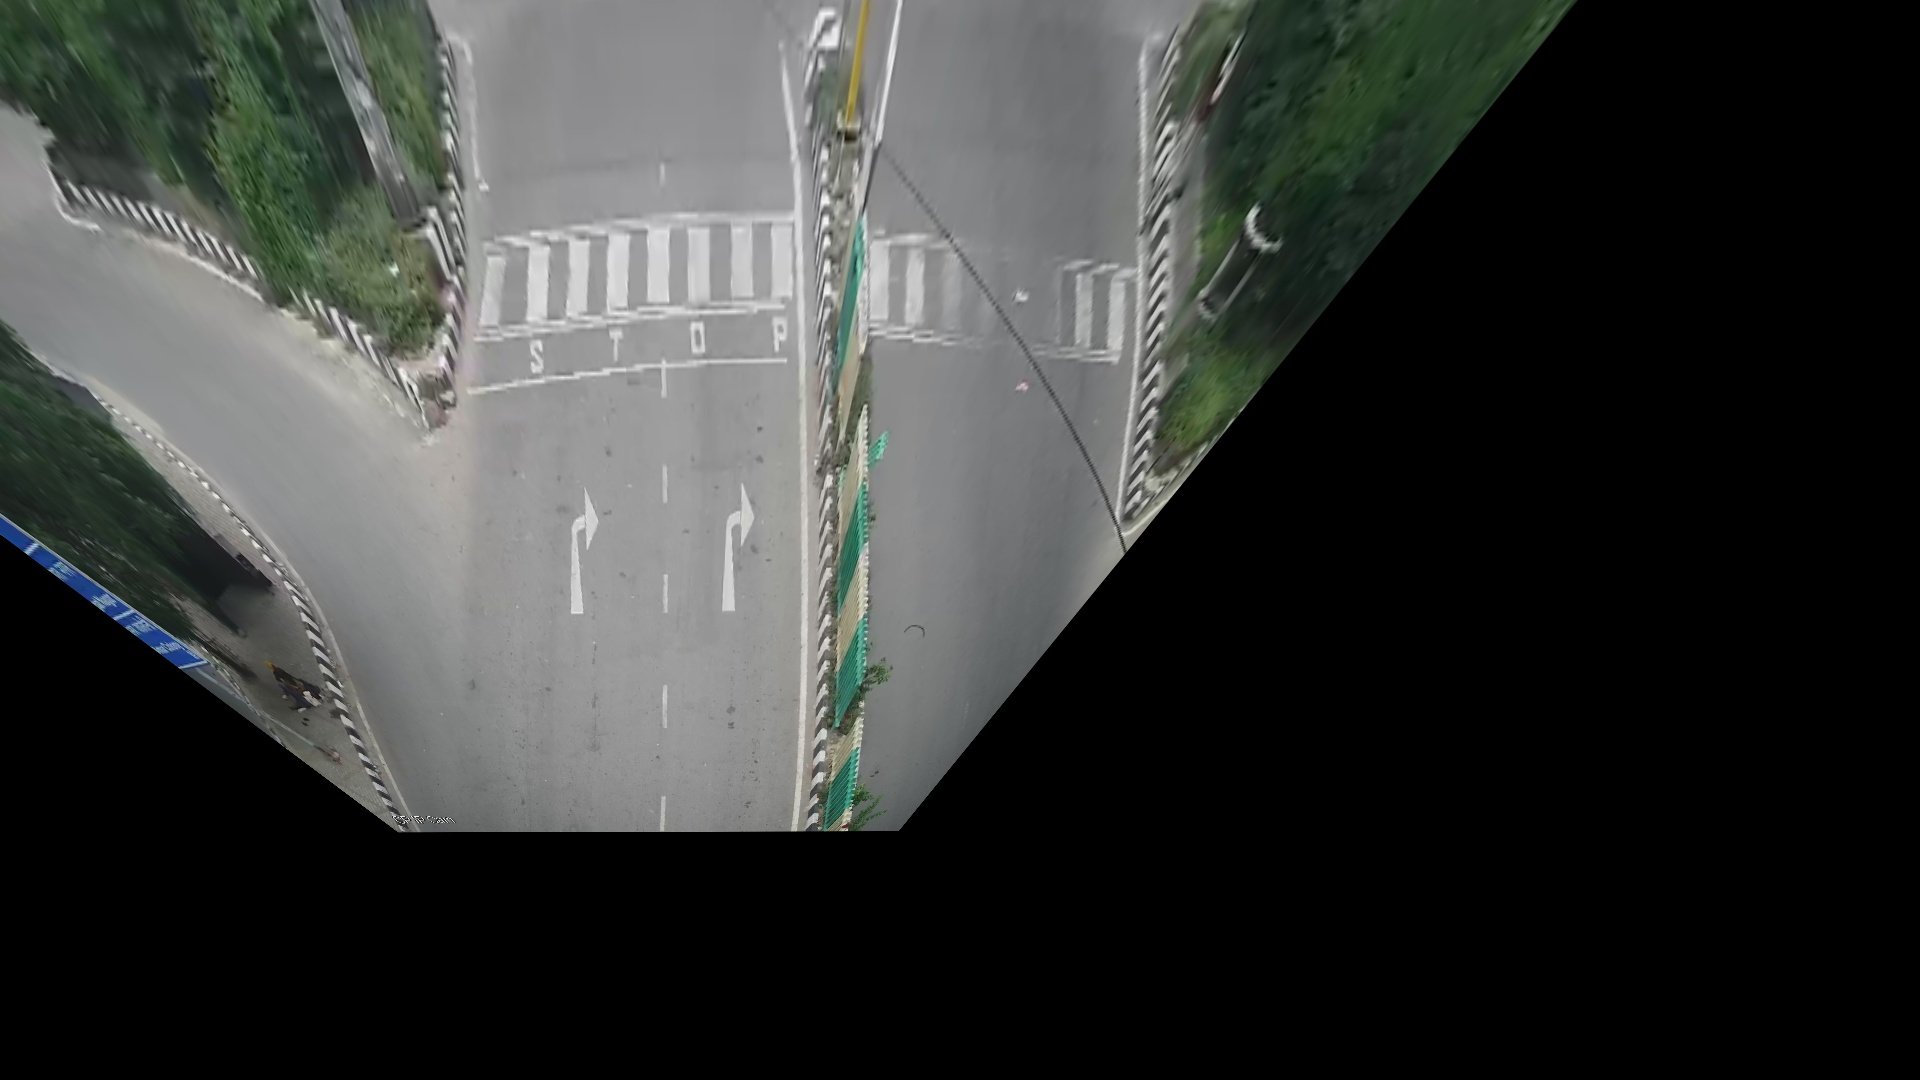
\includegraphics[scale = 0.19]{out_images/projected_out_empty.jpg}
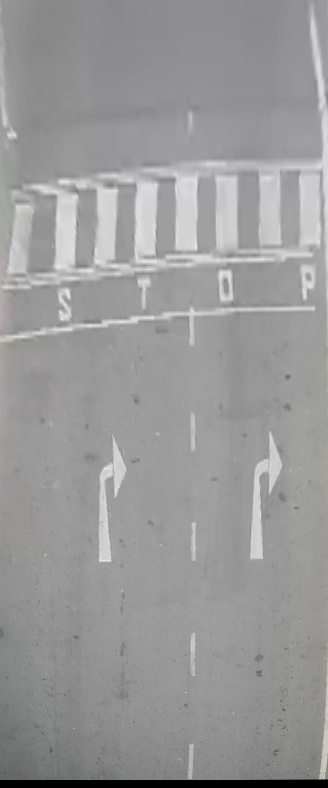
\includegraphics[scale = 0.26]{out_images/cropped_out_empty.jpg}
\\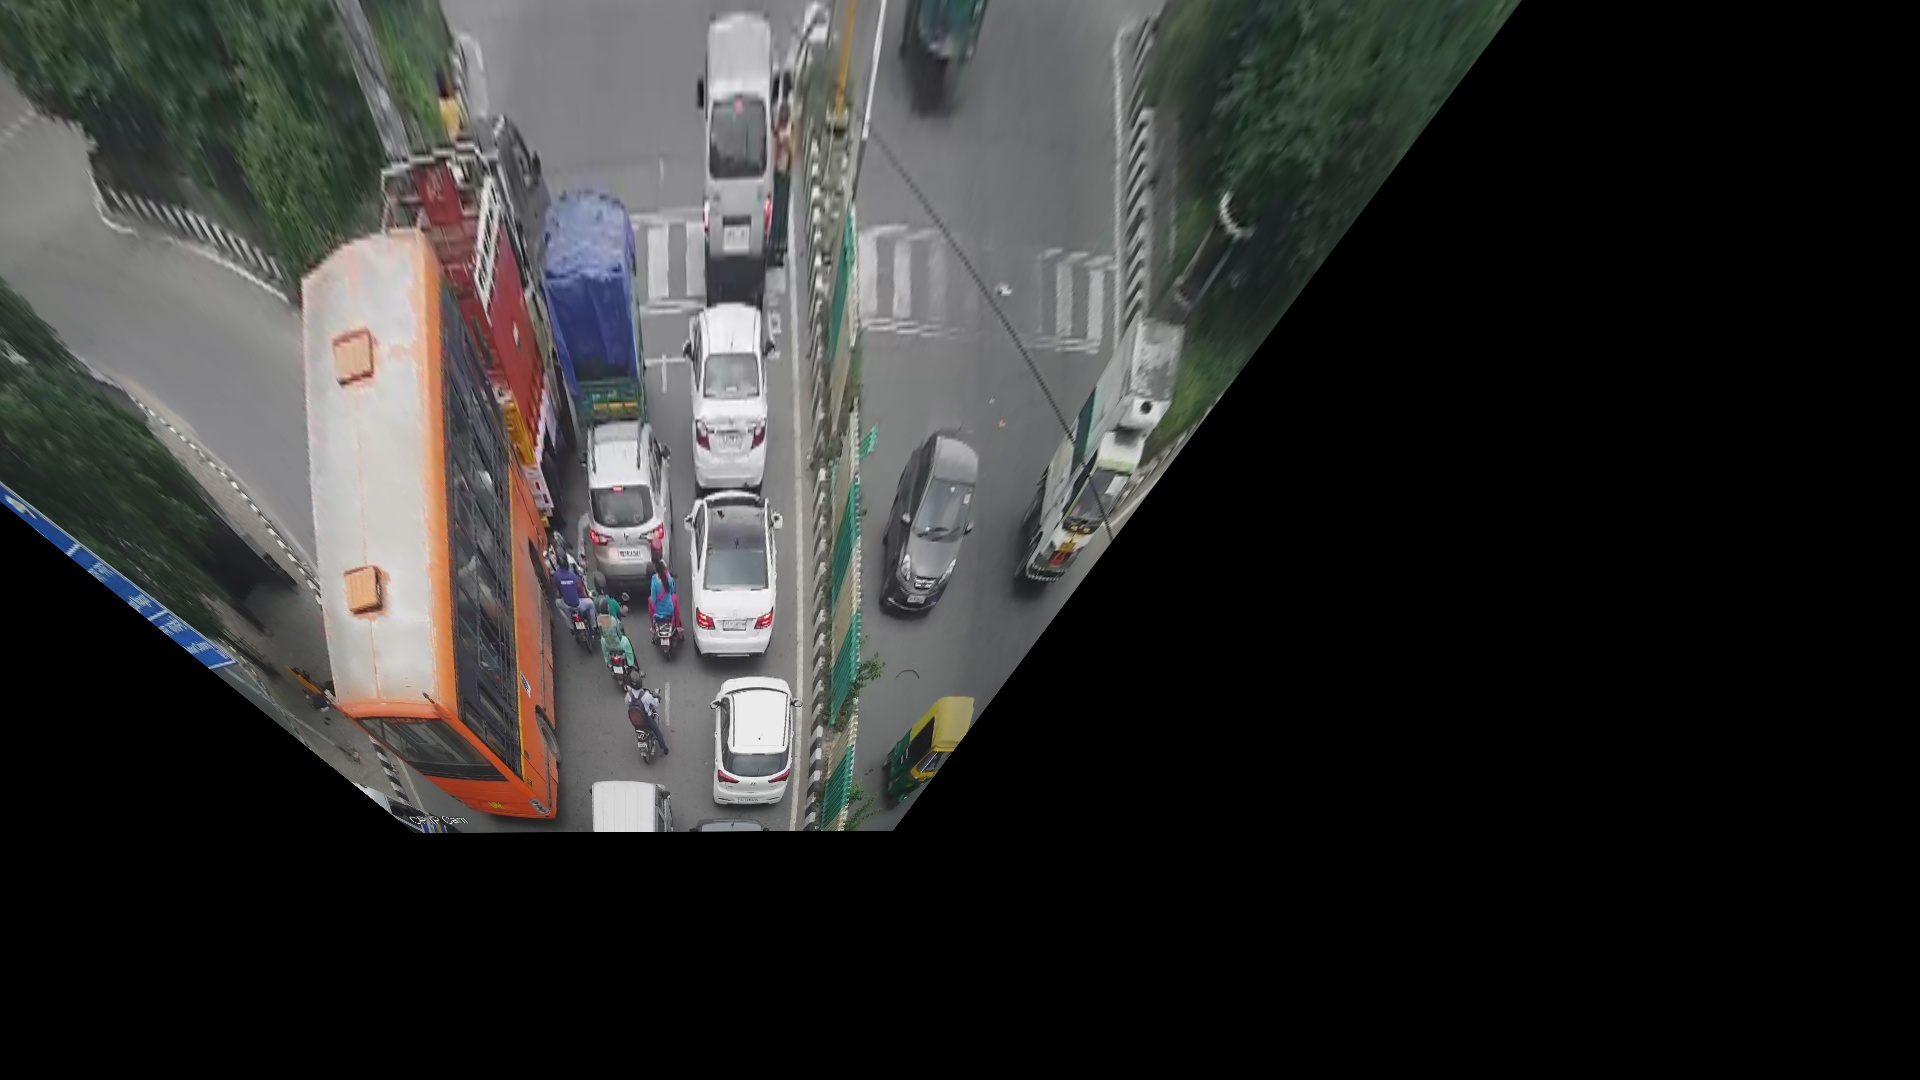
\includegraphics[scale = 0.19]{out_images/projected_out_traffic.jpg}
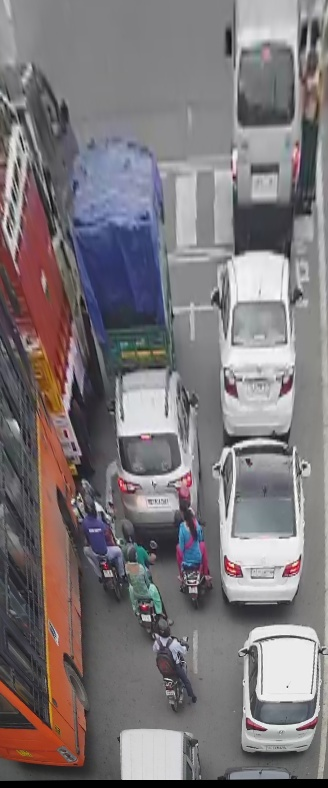
\includegraphics[scale = 0.26]{out_images/cropped_out_traffic.jpg}

\subsection{User Interface}
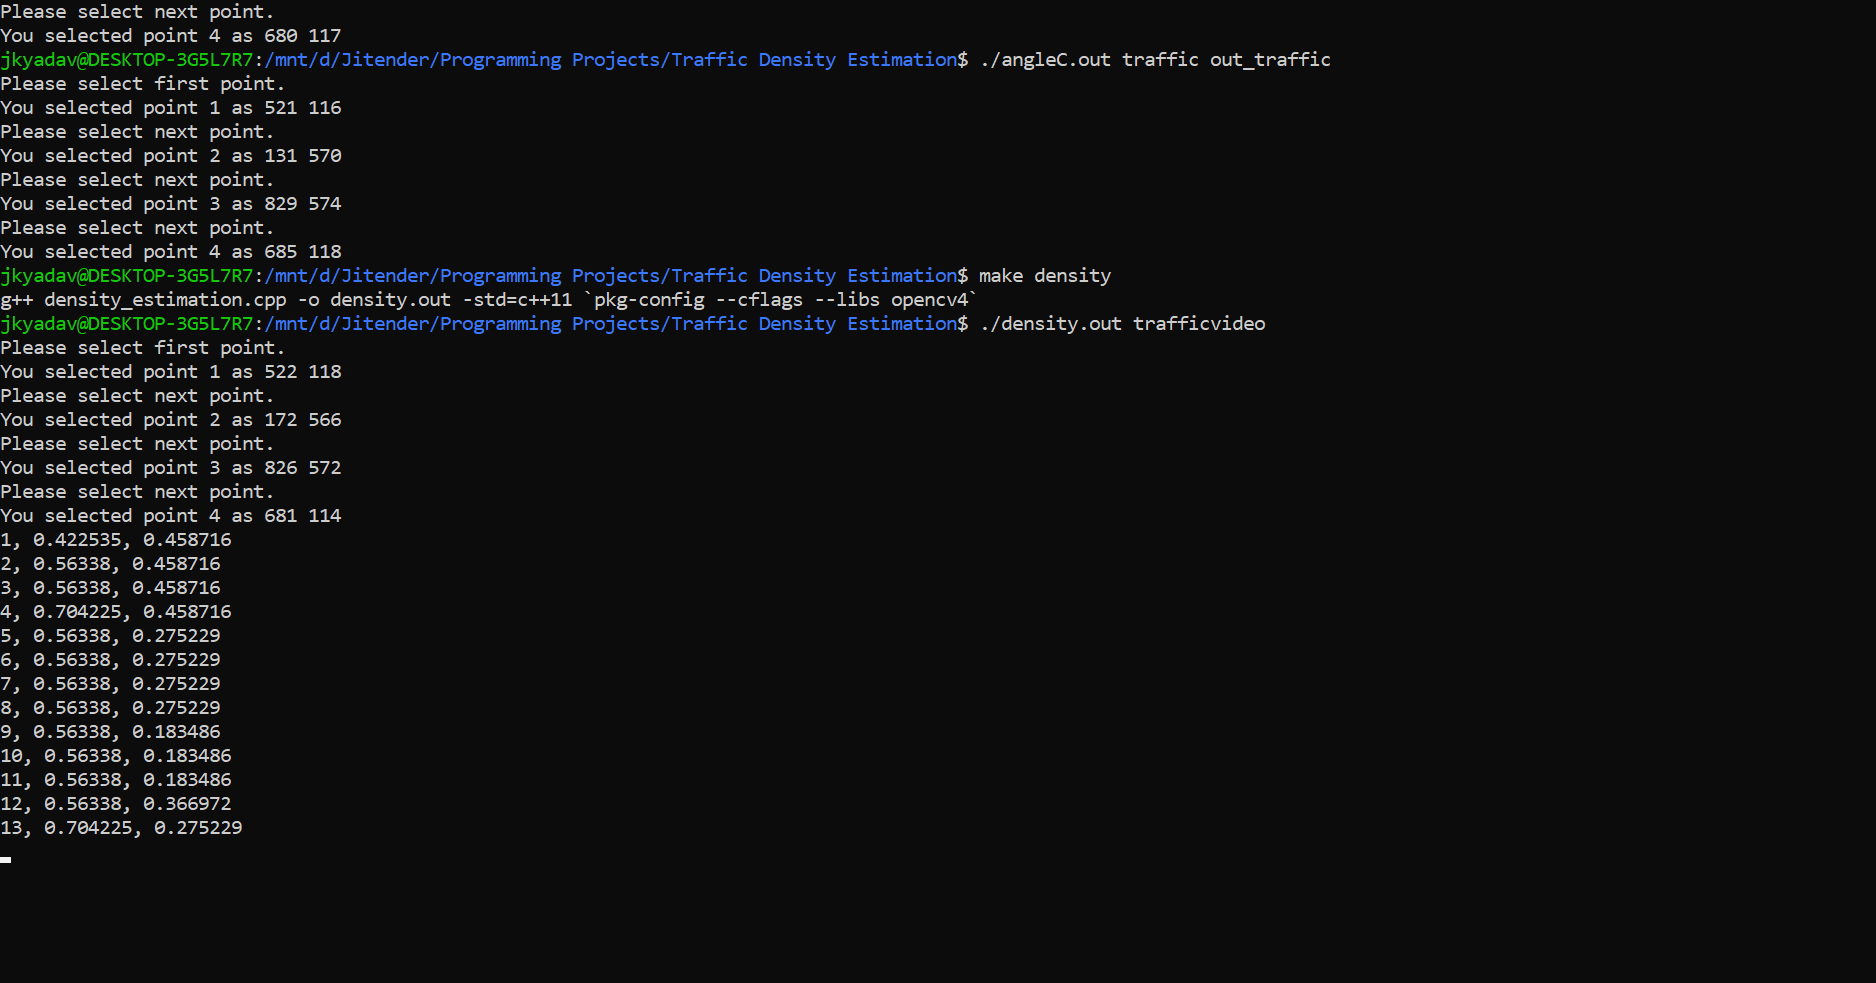
\includegraphics[trim = 0cm 4.5cm 13cm 0cm, clip=true, scale = 0.44]{user_interface/densityIO.png}
\vspace{2pt}
\\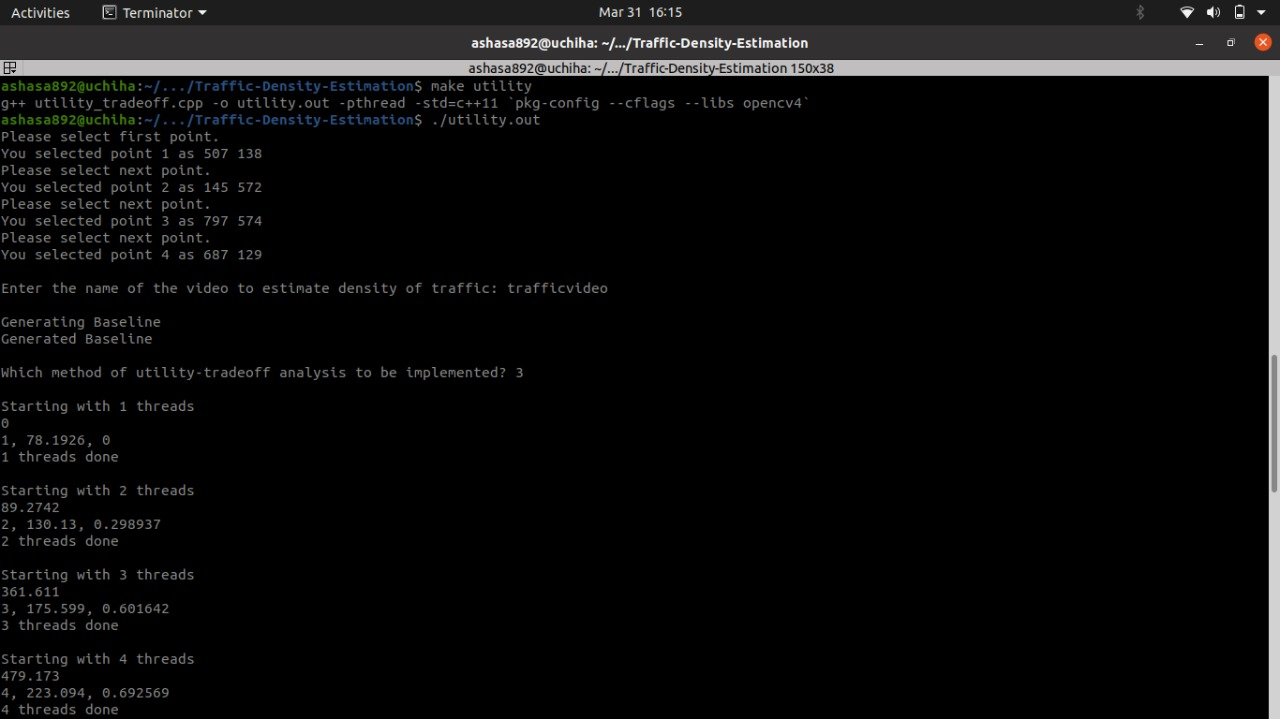
\includegraphics[trim=0cm 1cm 17cm 2.5cm, clip=true, scale = 0.57]{user_interface/utility_IO.jpeg}

\subsection{Queue and Static Density Curves}
When the output of the second sub-task was plotted using \textit{matplotlib} library of python, the following graph was obtained, which is similar in shape to the expected output for the given video.
\\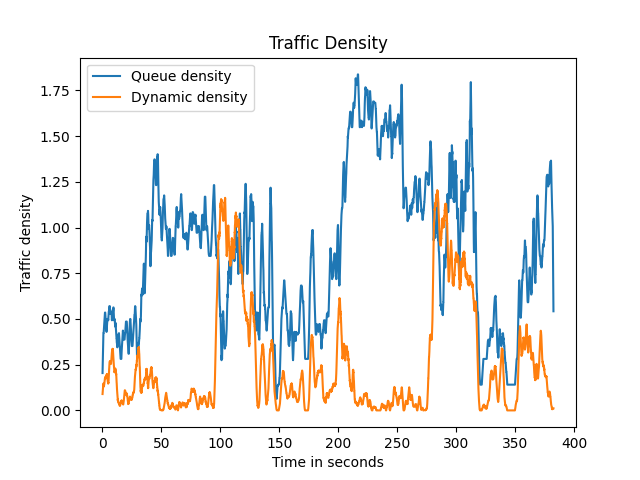
\includegraphics[]{out_images/out_graph.png}

\section{Utility Trade-Off Analysis}
As we try to optimize the program to work faster by changing one or more parameters, the amount of deviation from the expected output increases, that is, the utility of the program decreases. The utility has been measured as \textbf{the root mean square of the percentage deviations from the expected baseline output subtracted from 100}. The time for each operation and the utility was measured as the parameters were varied.

\subsection{Method 1: Skipping Frames}
Every $X^{th}$ frame of the video was processed for the queue and dynamic density. Thus the parameter was \textit{X} and the utility was measured. It was observed that when X was increases from 1 to 10, 20, 30, 40, ... 100 the utility on an average decreased from 100 to as low as 50. On the other hand time taken to process also decreased from 100 seconds to as low as 12 second. Clearly, decreasing X made the program faster as was expected since not all frames were processed, the accuracy of the output reduced.
\\The obtained variations of utility and execution time were plotted and found as shown.
\begin{center}
    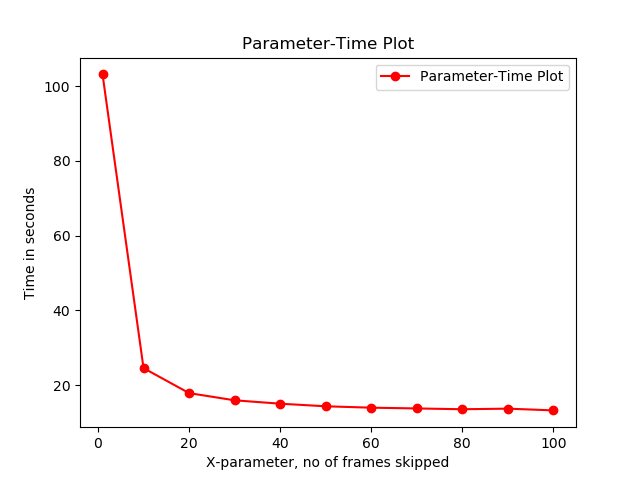
\includegraphics[scale = 0.9]{out_images/method_1_time.png}
    \\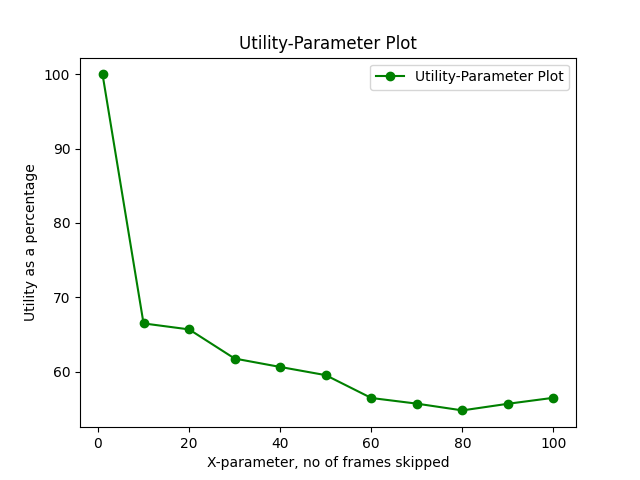
\includegraphics[scale = 0.9]{out_images/method_1_utility_param.png}
    \\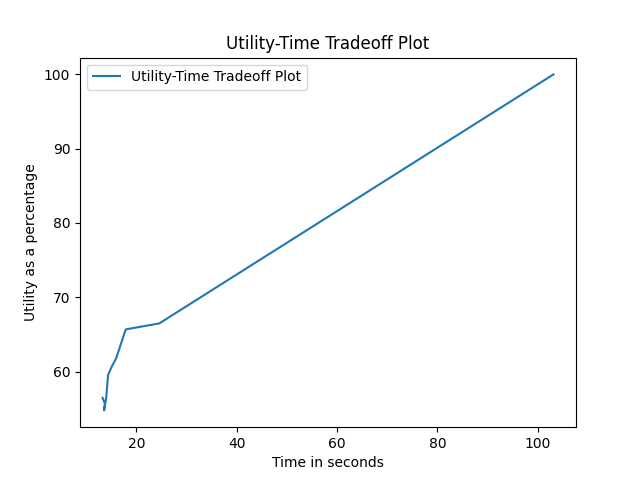
\includegraphics[scale = 0.8]{out_images/method_1_utility.png}
\end{center}

\subsection{Method 2: Varying Resolution}
The resolution of the original video was changed and the video was processed with lower resolution of each frame. When this was performed, it was observed that the utility dropped very fast with resolution while the time to process the frames did not change very significantly, though it also dropped with the resolution.
\\The plots of utility and time versus the parameter are as follows.

\begin{center}
    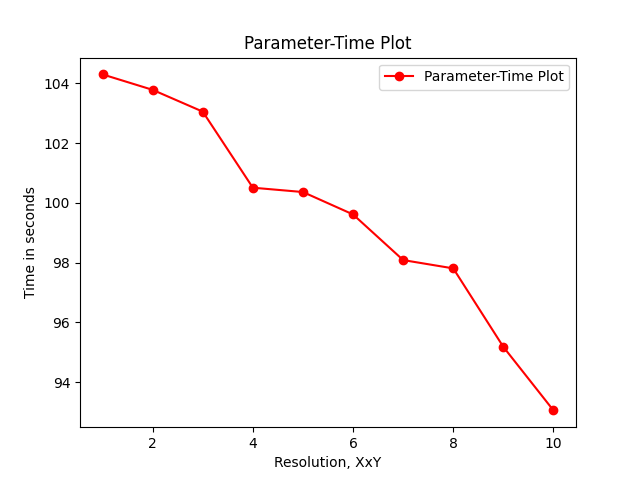
\includegraphics[scale = 0.8]{out_images/method_2_time.png}
    \\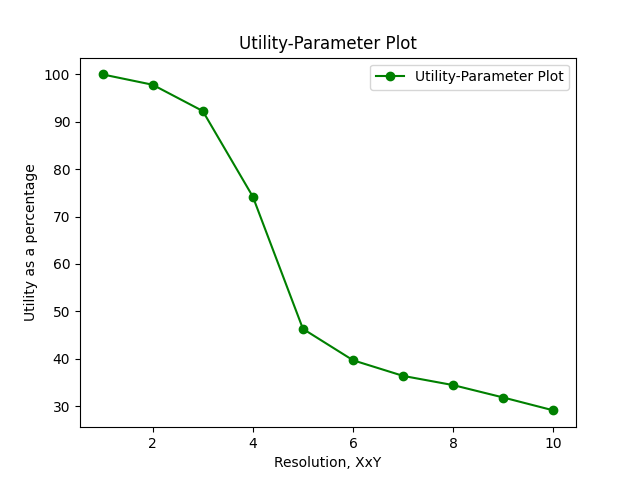
\includegraphics[scale = 0.9]{out_images/method_2_utility_param.png}
    \\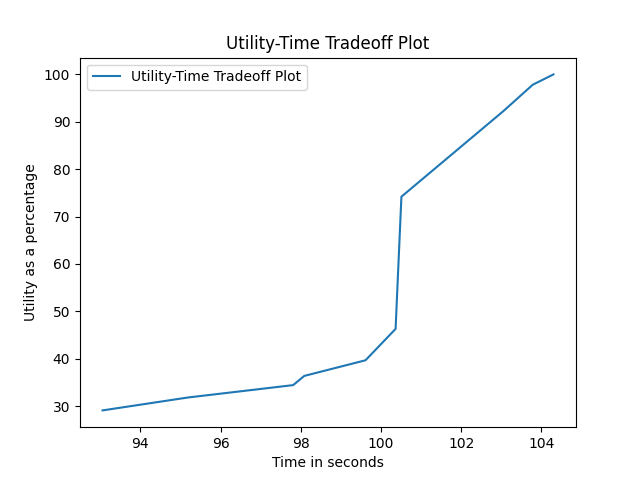
\includegraphics[scale = 0.9]{out_images/method_2_utility.png}
\end{center}

\subsection{Method 3: Spatial Distribution among Threads}
Each frame was divided into vertical parts and each part was given to separate thread. The results were then combined by adding the queue density values. It was observed that the utility reduced with the number of threads as expected, since a single vehicle could be spread among different threads. On the other hand, the execution time also increased with the number of threads contrary to expectations, since cropping of frames is itself a slow operation. Thus, utility decreased and execution time increased with the number of threads.

\begin{center}
    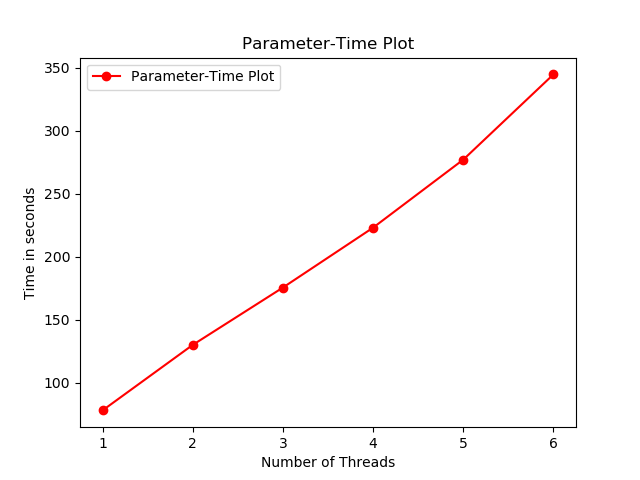
\includegraphics[scale = 0.8]{out_images/method_3_time.png}
    \\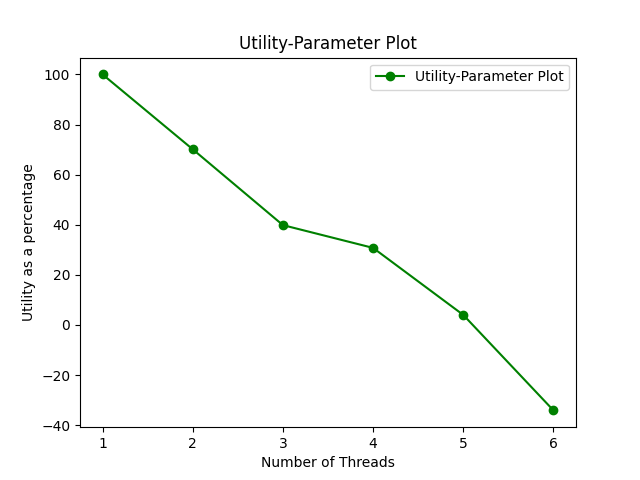
\includegraphics[scale = 0.8]{out_images/method_3_utility_param.png}
    \\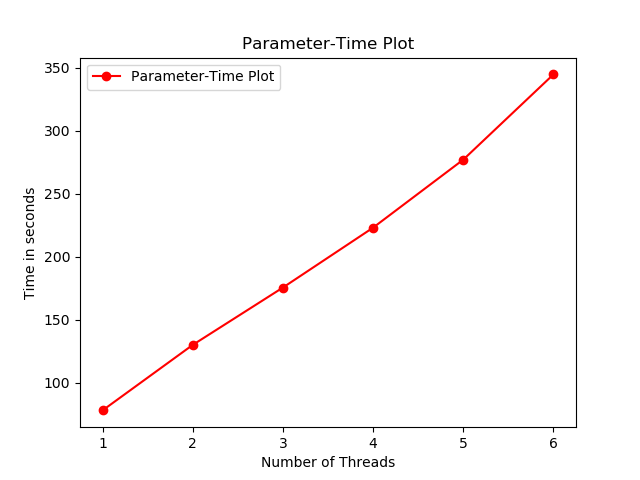
\includegraphics[scale = 0.8]{out_images/method_3_time.png}
\end{center}

\subsection{Method 4: Temporal Distribution among Threads}
The frames were divided into groups and each group was provided to a different thread to process. The utility was 100\% each time, since all the frames were processed accurately. On the other hand, the execution time reduced drastically with the number of threads as frames were processed simultaneously. The time taken to process was divided among the threads and harmonically reduced with the number of threads.

\begin{center}
    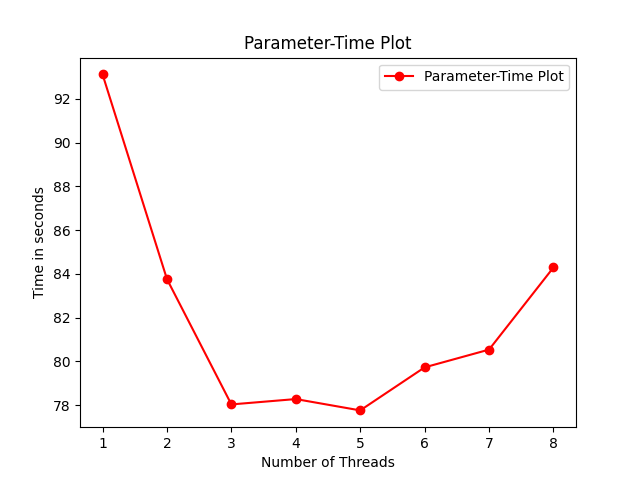
\includegraphics[scale = 0.8]{out_images/method_4_time.png}
    \\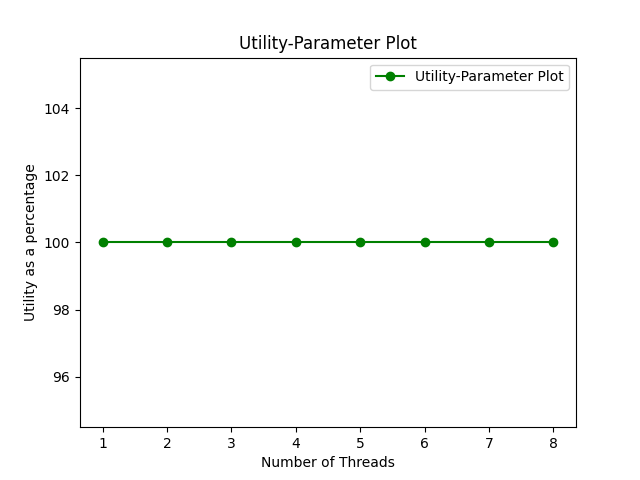
\includegraphics[scale = 0.9]{out_images/method_4_utility_param.png}
    \\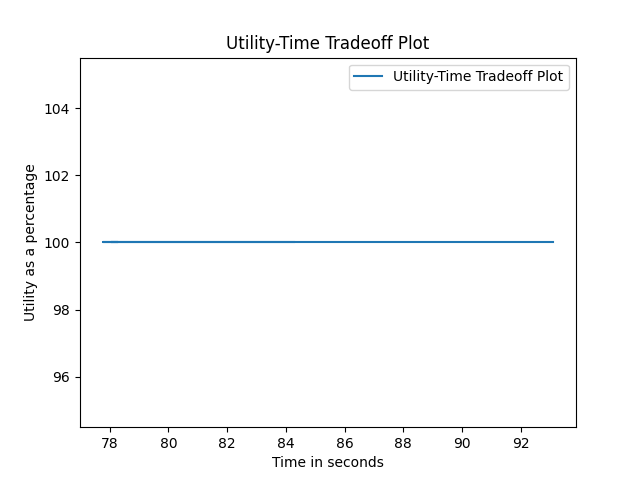
\includegraphics[scale = 0.9]{out_images/method_4_utility.png}
\end{center}

\subsection{Observations and Analysis}
The utility-time variations were studied for all the four methods and the following major observations were made.

\begin{itemize}
    \item[$\square$] In method 1, as the number of frames processed was reduced, the utility reduced drastically. On the other hand the processing time also decreased to a large extent.
    \item[$\square$] In method 2, as the resolution was decreased, the execution time decreased but the utility also decreased as the results were expected to be inaccurate.
    \item[$\square$] The method 3 was quite intriguing since with the use of more threads, the utility decreased (as the results were less inaccurate) but the processing time also increased.
    \item[$\square$] In method 4, the utility was maximum and constant at 100\% but the time decreased as the number of threads increased. But, the processing time was minimum at 8 threads and increased with further threads.
\end{itemize}

\begin{center}
    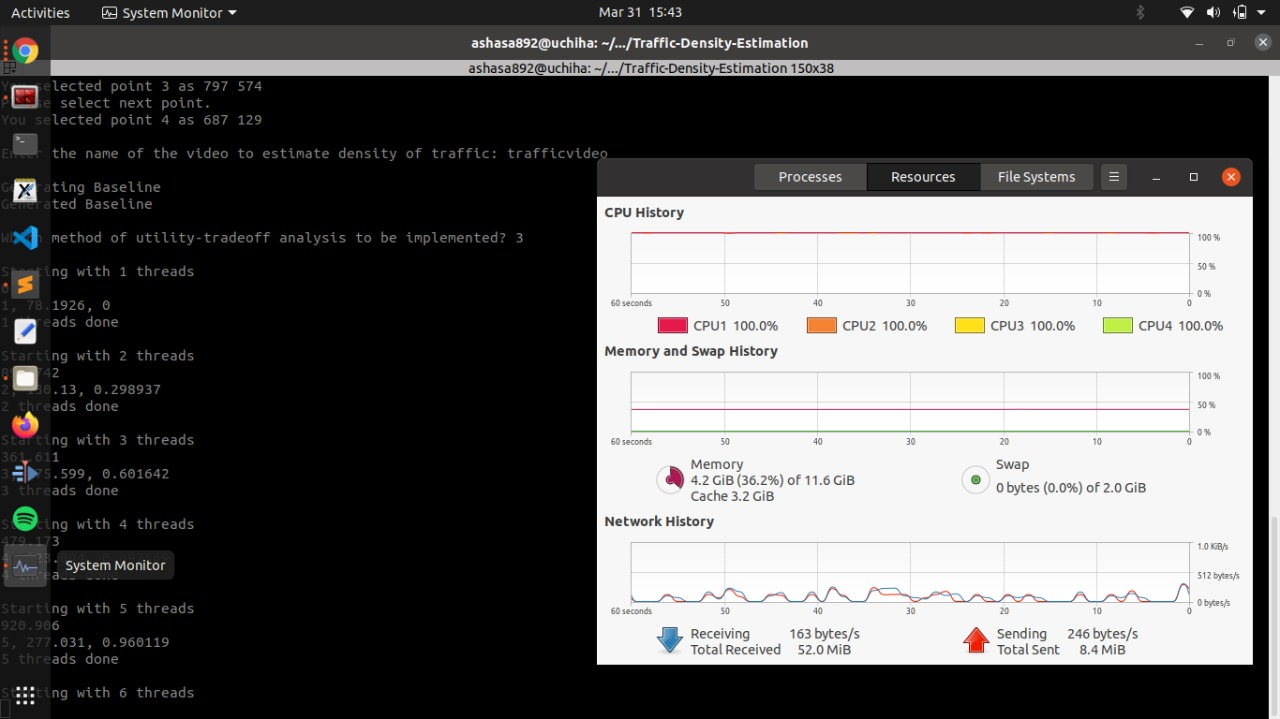
\includegraphics[scale = 0.36]{user_interface/CPU_Usage.jpeg}
\end{center}

The CPU usage was 100\% with the threads as shown in the following screenshot taken during the processing of frames using method 3.
\\Thus, it can be concluded that if we are to make a utility versus execution time trade-off, method 3 is definitely unsuitable as the execution time and error both increase. This is because, in case there is possibility of multi-thread usage, it is directly done by openCV. On the other hand, methods 1, 2 and 4 can be safely used to make such trade-offs.
\\Even among the three methods, method 4 is the most suitable since the execution time decreases and utility remains \textbf{constant at 100\%}. Thus splitting 8 threads to process some number of frames each leads to a lowering in execution time to a very large extent. This can be adopted for optimization.
\\On the other hand, if we compare the methods 1 and 2, we find subtle differences. In method 1, with the increase in value of X, the utility drops but the processing time also drops very fast as compared to method 2 where the processing time drops lesser and the utility drops to a very large extent, thus preferred method is reduction in number of frames processed.

\end{document}